%%%%%%%%%%%%%%%%%%%%%%% file typeinst.tex %%%%%%%%%%%%%%%%%%%%%%%%%
%
% This is the LaTeX source for the instructions to authors using
% the LaTeX document class 'llncs.cls' for contributions to
% the Lecture Notes in Computer Sciences series.
% http://www.springer.com/lncs       Springer Heidelberg 2006/05/04
%
% It may be used as a template for your own input - copy it
% to a new file with a new name and use it as the basis
% for your article.
%
% NB: the document class 'llncs' has its own and detailed documentation, see
% ftp://ftp.springer.de/data/pubftp/pub/tex/latex/llncs/latex2e/llncsdoc.pdf
%
%%%%%%%%%%%%%%%%%%%%%%%%%%%%%%%%%%%%%%%%%%%%%%%%%%%%%%%%%%%%%%%%%%%


\documentclass[runningheads,a4paper]{llncs}

\usepackage[colorlinks=true,linkcolor=black,citecolor=black,pdfnewwindow=true,urlcolor=blue,filecolor=blue,baseurl=./]{hyperref}
\usepackage{url}
\usepackage[utf8x]{inputenc}

% \newcommand{\mycite}[2]{\url{#1}{\cite{#2}}}
% \newcommand{\mycite}[2]{\url{#1}:\cite{#2}}
% \newcommand{\mycite}[2]{\href{http://twitter.com/home}{Twitter}.}
%\newcommand{\mycite}[2]{\href{./refs/#1}{\cite{#2}}}
\newcommand{\mycite}[2]{\cite{#2}}
%\newcommand{\myciteurl}[2]{\href{#1}{\cite{#2}}}


\usepackage{amssymb}
\setcounter{tocdepth}{3}
\usepackage{graphicx}

\usepackage{url}
%\urldef{\mailsa}\path|{alfred.hofmann, ursula.barth, ingrid.haas, frank.holzwarth,|
%\urldef{\mailsb}\path|anna.kramer, leonie.kunz, christine.reiss, nicole.sator,|
%\urldef{\mailsc}\path|erika.siebert-cole, peter.strasser, lncs}@springer.com|    
%\newcommand{\keywords}[1]{\par\addvspace\baselineskip
%\noindent\keywordname\enspace\ignorespaces#1}

\usepackage{color}
\usepackage[usenames,dvipsnames]{xcolor}
\usepackage{amsmath}
\usepackage[tight]{subfigure}
\usepackage{listings}
\definecolor{darkgray}{rgb}{0.2,0.2,0.2}

\lstset{language=c++,basicstyle=\scriptsize\sffamily,tabsize=2,framexleftmargin=5mm, frame=shadowbox, framesep=3pt,rulesepcolor=\color{darkgray},rulesep=.100pt,keywordstyle=\bf\color{blue},commentstyle=\color{magenta},stringstyle=\color{red},numbers=left,numberstyle=\tiny,numbersep=10pt,breaklines=true,showstringspaces=false,columns=flexible}

\newcommand{\tomas}[1]{{\color{red}{\textbf{Tom: #1}}}}
\newcommand{\stefan}[1]{{\color{magenta}{\textbf{St: #1}}}}
\newcommand{\christian}[1]{{\color{green}{\textbf{Ch: #1}}}}
\newcommand{\tobias}[1]{{\color{bleu}{\textbf{Tob: #1}}}}


\newcommand{\myvec}[1]{\ensuremath{\mathbf{#1}}}
\newcommand{\mymat}[1]{\ensuremath{\mathbf{#1}}}
\newcommand{\Vx}{\myvec{x}} % position vector
\newcommand{\Vv}{\myvec{v}} % velocity vector
\newcommand{\Va}{\myvec{a}} % acceleration vector
\newcommand{\Vdv}{\myvec{dv}} % change of velocity vector (unknown in implicit CG, and used in constraint solver)
\newcommand{\deriv}[2]{\frac{\partial #1}{\partial #2}} % Partial derivative


% \newcommand{\mysubsection}[1]{\noindent \textbf{#1: }}
\newcommand{\mysubsection}[1]{\textbf{#1: }}
% \newcommand{\mysubsection}[1]{\subsection{#1}}

%\usepackage{miseenpage}

\begin{document}

\mainmatter            % start of your contributions

\title{Simulation of Congenital Heart Defect Corrective Surgeries Using Thin Shell Elements}
%
%\author{Stefan Kislinskiy\inst{1}
%\and Tom\'{a}\v{s} Golembiovsk\'{y}\inst{2,3}
%\and Christian Duriez\inst{2}
%\and Eug\'{e}nie Riesenkampff\inst{4}
%\and Titus Kuehne\inst{4}
%\and H.-P. Meinzer\inst{1}
%\and Tobias Heimann\inst{1}}
%
%\institute{German Cancer Research Center (DKFZ), Heidelberg, Germany
%\and Inria, Lille, France
%\and Faculty of Informatics, Masaryk University, Brno, Czech Republic
%\and German Heart Institute Berlin (DHZB), Berlin, Germany}

\author{Anonymous}

\institute{Anonymous}

\maketitle

\begin{abstract}
Pediatric cardiac surgery is particularly challenging because the final decisions on the procedure choice take place at the last minute.
The work presented in this paper aims at proposing an interactive software dedicated to preoperative planning.
This new tool would permit to evaluate several possible surgical procedures on a virtual anatomy of the patient and anticipate the decisions.
The surgery involves a reconfiguration of the blood vessels that are close to the heart.
During the surgery, the vessel walls are deformed, cut, and reconnected to other vessels or closed with an artificial patch.
We propose to anticipate the geometry changes of the vessel walls using a simulation based on thin-shell elements.
We demonstrate that our approach allows for simulating the results of low-level surgical procedures, with a unified strategy for joining the vessel models and simulate their subsequent behavior.

\end{abstract}

\section{Introduction}
Surgical interventions in infants with congenitally malformed great arteries and hearts are extremely challenging due to the complex and heterogeneous nature of their disease pattern. Cardiac surgeons rely on non-invasive imaging for patient-specific examination and possible appropriate surgical procedures may be sketched conceptually in advance, but the most promising approach is often chosen just in time during the actual open-heart operation. This is the first time the surgeon gets a concrete idea of possible outcomes for different surgical procedures. His decision has to be made in short time and is still based heavily on imagination capabilities and experience.

To improve planning of such pediatric cardiac surgeries it is possible to create 3-dimensional heart models out of acquired image data REF and to use them as input for surgical simulation systems. However, most present simulation systems focus on low-level surgical procedures, i.e. performing actual incisions and suturing with special input devices in real-time REF. Their purpose is either by means of educational training or planning access strategies to reach the malformations of the heart or great arteries. In such {\itshape reactive} simulation systems it is more important to enable simulations in real-time than to simulate tissue and blood vessels in a physically accurate manner.

To be able to predict the result of complex surgical procedures, a physically correct simulation is mandatory. REF present a {\itshape predictive} surgical simulation system for bidirectional Glenn shunts and basically similar surgeries. They use a hybrid model to simulate deformations of blood vessel trees by binding a surface mesh to a reference Cosserat rod REF elastically. While the mesh models surface details of blood vessels, the Cosserat rod models global deformations, i.e. stretching, bending, twisting and shearing. Joining of blood vessels end-to-end or end-to-side is realized by attaching contracting springs. This approach adds surplus energy to the physical system and special care has to be taken during the simulation to compensate for that. The software performs low-level surgical procedures automatically with only a minimum of interaction required which allows the surgeon to focus on the actual overall surgical procedure. Given the input of the surgeon, a complete simulation takes only seconds to produce a predictive result for further examination and evaluation of possibly undesired collisions or deformations of blood vessels. Although the results are promising, the method is limited to operations on uniform tubular structures that do not change their surface arbitrary. Surgical procedures heavily changing surface details of blood vessels, i.e. arbitrary shaped patches for correction of complicated coarctations and stenosis, are not possible with this hybrid model since the physical behavior of blood vessels is simulated by the Cosserat rod and its {\itshape binding} to the surface mesh.

In this paper we present an alternative, improved approach using a simulation model solely based on elastic thin shell elements. Our method is not limited to well-formed blood vessels and captures all low-level procedures necessary for aortoplasty. By using a relaxation process we can arbitrarily join or attach blood vessels and patches without using springs that would add surplus energy to the physical system. We prove that simulation time is still reasonable or even decreased by taking special care of the overall tubular structure of blood vessels during generation of thin shell elements.
%TODO: Include only a few sentences to CHD in general.
%
%Surgical interventions in infants with congenitally malformed great arteries and hearts can be difficult due to their disease pattern's complex and heterogeneous nature. Today, patient-specific 3-dimensional heart models can be acquired by modern techniques of non-invasive imaging and image post-processing [REFERENCE]. Nevertheless, cardiac surgeons tend to rely solely on subsets or 2-dimensional views of obtained 3-dimensional image data for examination. Possible appropriate surgical procedures may be sketched conceptually and the most promising approach is chosen just in time during the actual open-heart operation. 
%\christian{to modify [ }
%This is the first time the surgeon gets a concrete idea of possible outcomes for different surgical procedures. 
%However, his decision has to be made in relatively short time and can still be based heavily on imagination capabilities and experience.
%\christian{  ] }
%
%
%To improve planning of these kind of cardiac surgeries, obtained 3-dimensional heart models could be used as input for patient-specific surgical simulation systems. 
%
%\christian{not sure this is the right place for the following paragraph (It begins the state of the art while the work is not yet introduced) : [}
%Present simulation systems \christian{what simulation systems are we talking about ?}  focus on low-level surgical procedures [REFERENCES], i.e. performing actual incisions and suturing with special input devices in real-time. 
%Their purpose is either by means of educational training or planning access strategies to reach the heart's or blood vessel's malformations. 
%It is more important in such \emph{reactive} simulation systems to enable simulations in real-time than to simulate tissue and blood vessels in a physically accurate manner.
%\christian{ ] }
% 
%
%\christian{I think we should present our work as a continuity of what was proposed with the Cosserat model. We should reduce the discussion about this paper and show what is improved by our approach.}
%To be able to predict the result of complex surgical procedures, a physically correct simulation model must be used. 
%[REFERENCE] present a \emph{predictive} surgical simulation system for bidirectional Glenn shunts and basically similar surgeries. 
%They use a hybrid model to simulate deformations of blood vessel trees by binding a surface mesh to a reference Cosserat rod elastically.
%While the mesh models surface details of blood vessels, the Cosserat rod models global deformations, i.e. stretching, bending, twisting and shearing. 
%Low-level surgical procedures are done automatically by the software with only a minimum of interaction required which allows the surgeon to focus on the actual overall surgical procedure. 
%Furthermore the authors show that they can attach triangular shaped patches at loose ends of dissected vessels to allow joining of vessels with different circumferences. 
%Given the input of the surgeon, a typical simulation takes only seconds to produce a predictive result for further examination and evaluation of possibly undesired collisions or deformations of blood vessels. 
%Although the results are promising, the author's method is limited to uniform tubular structures and operations on them, i.e. joining blood vessels end-to-end or end-to-side. 
%Connection of blood vessels is done by using springs. 
%This approach introduces surplus energy to the physical system and special care has to be taken during the simulation to compensate for that. 
%Surgical procedures heavily changing surface details of blood vessels, i.e. arbitrary shaped patches to correct complicated coarctations and stenosis, are not possible with this hybrid model because the blood vessel's physical behavior is simulated by the Cosserat rod and its \emph{binding} to the surface mesh. 
%The authors state that more sophisticated physical models including finite element methods and thin shell elements would allow this but are computationally too expensive to produce results in reasonable time.
%
%
%\christian{\sout{In this paper we present an alternative}   Precisely, I propose to place our paper as an improvement of their approach } , universal approach using a simulation model solely based on elastic thin shell elements. 
%Our method is not limited to well-formed blood vessels and captures all low-level surgical procedures necessary for aortoplasty. 
%By using a relaxation process we arbitrarily join or attach blood vessels and patches anywhere without using springs that would add surplus energy to the physical system. 
%We prove that simulation time can be expected to be still reasonable or even decreased by taking special care of the blood vessel's overall tubular structure during generation of thin shell elements.
%
%TODO: Structure of Paper.
 

\section{Blood Vessel Model}
From our point of view, there are several requirements that the model
should be able to fulfill. Namely:

\begin{itemize}
  \item good support for deformations by bending and twisting
  \item the results of the deformation should be global
  \item method should allow arbitrary models and not rely on specific
  structure of the object (e.g. on tubular structure like \cite{Li2009})
  \item the model has to be able to deal with collisions (e.g. between the
  aortic arch and pulmonary artery)
\end{itemize}

Several different models are commonly used for modelling thin structures or
tubular-like structures resembling blood vessels. \tomas{Add refs. or
reformulate!} For the predictive simulation of the surgery we choose to use
thin shell elements, because in our opinion it satisfies all the
requirements very well. They are very often considered numerically too
expensive, this is however not necessarily true.

\tomas{image: single shell}

The formulation of the thin shell elements is based on the mechanics of
continuum. These elements are commonly used in physics and mechanics for
deformation modelling of thin structures because they are numerically more
stable then volumetric FEM methods in this situation. The shell element is
a 2-dimensional element whose thickness is a parameter of the simulation.
Often the thickness is considered constant over the surface of the element.
Shell combines forces from in-plane deformations, like stretching or
shearing, with bending forces. Such internal forces $\myvec{f}$ are a
function of current displacement measured as difference of current shape
$\myvec{x}$ from the rest shape $\myvec{x_0}$.

\begin{equation}
  \myvec{f} = K(\myvec{x} - \myvec{x_0})
\end{equation}

For more thorough description we refer the reader to the textbook about
Finite Elements for example \tomas{add ref}.

In the rest of the section we want to show that the performance of a model
based on the shell element is adequate for the simulation.

\begin{figure}[tbh]
  \begin{minipage}[b]{0.3\linewidth}
      \framebox[1cm]{\rule{0pt}{1cm}}
      %\includegraphics[width=\columnwidth]{img/}
      \caption{Bending shell element}
      \label{fig-shell}
  \end{minipage}
  \hspace{0.1\columnwidth}
  \begin{minipage}[b]{0.6\linewidth}
    \centering
    \begin{tabular}{cc}
     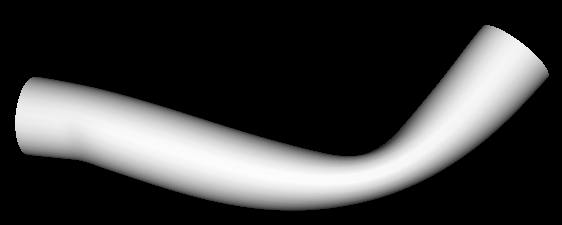
\includegraphics[width=0.5\columnwidth]{img/compare-bend.png}
      &
      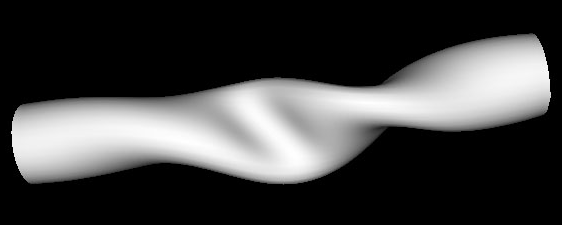
\includegraphics[width=0.5\columnwidth]{img/compare-twist.png}
      \\
      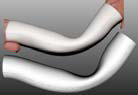
\includegraphics[width=0.5\columnwidth]{img/compare-bend-other.png}
      &
      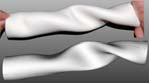
\includegraphics[width=0.5\columnwidth]{img/compare-twist-other.png}
    \end{tabular}
    \caption{Bending and twisting deformations. Upper: shell model; middle:
    artificial tube, bottom: Cosserat rod \cite{Li2009}. (Credits for the
    bottom images: Li et al.)}
    \label{fig-deformations}
  \end{minipage}
\end{figure}

Figure \ref{fig-deformations} shows different deformations that are likely to
occur during the surgery (bending and twisting). The figure compares our
results with the results of Li et al. \cite{Li2009}. As you can see the
results are closer to the real deformations.

The bending property of the shell allows us to use smaller number of
elements for the simulation and use high polygonal model only for
visualisation. The convergence of the model is a key factor here. In our experiments we
were able to use only as few as eight nodes around the circumference of a
tubular model while still maintaining realistic behaviour. Figure
\tomas{add-ref} shows the results for different number of nodes along the
circumference.

\tomas{image: convergence}

We have used the model of Olivier Comas \cite{Comas2010b,Comas2010c} and
also our own model. But our method described in section \ref{sec-method}
does not depend on any particular model. Since we use the method as a
geometrical tool we have also certain independence on physical parameters.
For example the variation of Young's modulus in the interval from $10^3$ to
$10^7$ resulted to only $0.1\%$ change of the deformation.


% vim: et sw=2 tw=75 fdm=marker fdc=2 spell


\section{Simulation of Low-Level Surgical Procedures}
\label{sec-method}
In order to repair malformations of the great arteries surgeons perform several low-level procedures on blood vessels. These include arbitrary incisions, resections of whole blood vessel parts, attaching patches and reconnection of blood vessels end-to-end or end-to-side. From a technical view, all cutting operations can be done prior to simulation by splitting shell elements along their edges which correlates to the actual incision. New shell elements can be added to a mesh or rearranged to align their edges along an incision. On the contrary, joining and suturing of blood vessels and patches typically deform blood vessel walls to a certain amount which has to be simulated. Recent simulation systems \cite{Sorensen2006,Mosegaard2004,Li2009} realize suturing through attachment of contracting springs that have no physical correlation. Springs introduce surplus energy to a physical system and special care has to be taken during simulation to compensate for that.

\begin{figure}[tbh]
\begin{center}
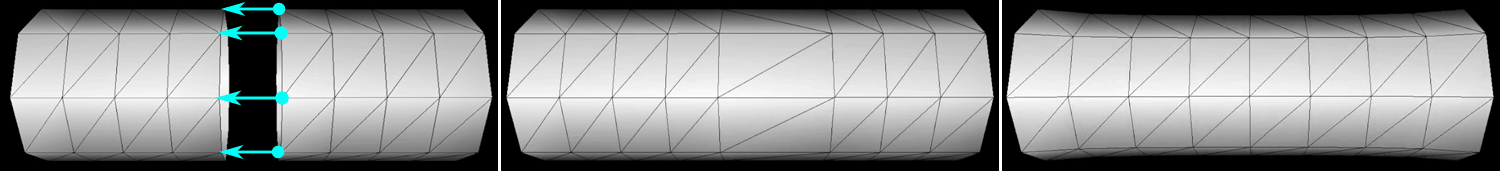
\includegraphics[width=\columnwidth]{img/new-joining.png}
\end{center}
\caption{Joining of thin shell element meshes. Left: Split meshes. Center: Shell elements along the joining edges are connected. Right: Final result after the simulation.}
\label{fig-JoiningVessels}
\end{figure}

We present a new approach that overcomes these difficulties by performing topological changes on the mesh to connect shell elements along joining edges (see figure \ref{fig-JoiningVessels}). Since there is a certain distance between two joining edges in general, a topological modification alters the shape and size of affected shell elements. Note that in this simulation state there is temporarily no correlation to reality. We then start a controlled relaxation process during which the shell elements progressively converge to their energetical equilibrium. To keep the simulation stable we avoid a strong increase in internal forces by linearly interpolate the rest shape of the connected mesh to the initial rest shape before joining. The effect is similar to contracting springs but there is no such problem like surplus energy after the joining process is done.

% The primary goal of the surgery is to restore a normal heart function and circulation.
% This goal is reached by rebuilding the heart in a more or less anatomical way.
% There are several types of low-level task the surgeon usually employs while
% performing the surgery that are:

% \begin{description}

  % \item[End to end aortoplasty:] the surgeon completely cuts away the
    % affected part of aorta and sutures the two ends of aorta back together.

  % \item[Patch aortoplasty:] the surgeon performs a cut along the axis of
    % the aorta thus allowing the narrow place to expand. Then applies a
    % patch from artificial material to fill the hole in.

  % \item[Subclavian flap aortoplasty:] the nearest artery is cut,
    % removing also half of the artery (along the axis) and part of the
    % aorta in the affected place. He then uses the rest of the artery to
    % patch the aorta.
    
  % \item[Reconnection and joining of blood vessels:] In addition to the modification of the aorta, the surgeon is lead to establish certain connections that are absent in pathological anatomy.

% \end{description}

% With our method we are able to simulate these tasks, in order to be able to plan them.
% We have based our general approach on a common characteristic: In all these operations the surgeon sutures two or more edges of the vessel walls together.
% Since we are interested in predicting the results rather than creating a training simulator for suturing (trained surgeon knows well how to perform the sutures) the simplest way of performing the suture would be to connect the respective edges with springs. 
% Springs however adds some unwanted energy to the system. 
% Our method is based on a topological connection of the shell elements that are neighbors of the joining edges and a controlled relaxation of these shell elements' rest shape.

% We start with a mesh representing the situation after all the cuts have been performed but before suturing takes place. 
% In the first step we perform the required topological changes to the mesh. We keep the number of elements in new mesh the same as in the original mesh so that we can define 1:1 mapping between elements of these meshes.
% The Figure \ref{fig-JoiningVessels} (a) and (b) explains this operation when joining vessels. 
% Then we start the simulation on the modified mesh while keeping the information of the original rest shapes of all shell elements. 

% \begin{figure}[tbh]
% \begin{center}
% 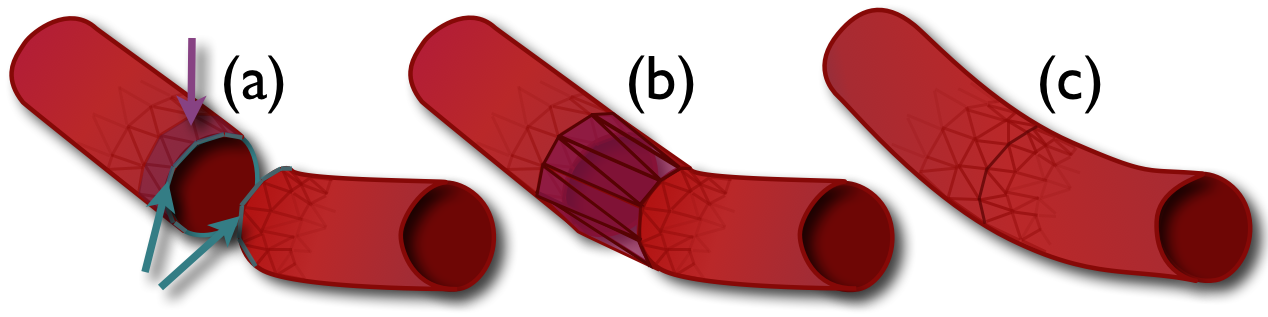
\includegraphics[width=\columnwidth]{img/rest_shape_scheme.png}
% \end{center}

% \caption{Scheme showing the method for joining two vessels \stefan{Isn't that example too complex? I think it is really hard to actually see what is happening here. At least the colors have to be changed because the different layers are colored quite equally and it should be zoomed in to the interesting area were the joining takes place. Remember also that the procedings are printed in black and white and that everything must be visible when printing out this figure black and white. There must be way more contrast.}:  (a) the cut on vessel meshes is performed in a 3D geometry edition software. In the software, we impose that the number of the segments on the edges is the same on both side  (\color{BlueGreen}{$\mathbf{\rightarrow}$}\color{black})
% Moreover, we select some shell elements that lie along the sutured edges (\color{purple}{$\mathbf{\rightarrow}$}\color{black}).
% (b) In our software, we connect the vessel topologies by performing a relaxation of the shape and the rest shape for the selected shells.  
% (c) We progressively re-contract the rest shape of the shells while computing the deformation of the whole unified mesh. 
% In the final steady state computed in the simulation, the shell elements have all their correct rest shape.}
% \label{fig-JoiningVessels}
% \end{figure}

% We can not always step back all the shells to their original shape (transition from figure \ref{fig-JoiningVessels} (b) to (c))  in a single simulation step. 
% In case of non-small distance between the nodes that are sutured together, the involved elements will undergo large deformation that could create quick and non-smooth increase of internal forces and  cause unwanted effects.
% To allevieate the problem we have implemented the technique that allows for moderate changes in the rest shape between simulation steps.
% Between the start and the end of the simulation we use a linear interpolation of the rest shape for the shells that lie along the sutured edges. 
% The interpolation starts with the rest shape equal to the deformed elements and we progressively lead the elements to recover their original rest shape.
% This way, the simulation gradually forces the side edges to connect without any abrupt jump in the behavior.
% When all elements have recover their original rest shape, the steady state found in the simulation corresponds to a physics-based energetical equilibrium of the shells deformation. 
% Thus, we take these positions as an estimation of the result of the connection of the vessels.


\section{Results and Discussion}
\section{Results and Discussion} %{{{
As the first step, we evaluate the influence of the Glisson's capsule on the mechanical response of the tissue during
the aspiration test. 
In~\cite{Hollenstein2006} it is reported that the influence of the capsule is significant, as modeling 
only the parenchyma without considering the membrane results in overestimation of the deformation by a factor of 2 to 3. 
In order to verify this observation, we performed a simulation using capsule parameters measured experimentally on 
ex-vivo pig liver~\cite{Umale2011}: Young's modulus of the membrane was set to $E_c$=8.22\,MPa and thickness was
$t_c$=20\,$\mu$m. 
Since the values for parenchyma elasticity reported in the literature vary significantly being usually reported between 2\,kPa to 5\,kPa, 
we employed a value $E_p$=3.5\,kPa for the Young's modulus of the parenchyma. 

In Fig.~\ref{fig-aspiration2} the profiles of cuts in the middle of the
test cube are presented showing significantly larger deformation in the model without capsule assuming that the same negative pressure was applied 
on the tissue surface inside the tube. Moreover, it can be observed that the deformation without capsule is overestimated by a factor 
close to 2, which is in perfect agreement with the results reported in~\cite{Hollenstein2006}.
Fig.~\ref{fig-aspiration3} presents the evolution of displacement in time at central node on the cube surface. The effect of increased combined stiffness is clearly visible.

In the second step, we employed the simulation to reproduce the displacements values obtained via simulation in~\cite{Hollenstein2006,Nava2008}.
Whereas the simulation in the referenced work was done on a mesh composed of tetrahedral elements for both the parenchyma 
and the capsule, we modeled the capsule using the triangular elements as shown in section~\ref{ss:capsuleModel}.

Since the Young's moduli of neither parenchyma ($E_p$) nor capsule ($E_c$) were specified exactly, we obtained both as follows: first, 
we performed a set of simulations without the capsule for different values of $E_p$: the value that provided a good match 
with reported displacements was $E_p$=30\,kPa. 
Then, we fixed the thickness of the capsule to be $t$=93\,$\mu$m (reported as the average value in the paper) and 
using $E_p$=30\,kPa, we ran the simulation repeatedly using the model with the capsule. In each simulation we 
used different value $E_c$ of the Young's modulus for the capsule in order to minimize the displacement error w.r.t. the 
reported values. The minimal value of error (not exceeding 1\%) was obtained for $E_c$=3\,MPa. This 
value lies in the range of capsule elasticity coefficients reported by experimental measurements.

%Moreover, we are able to reproduce
%the measurements presented in~\cite{Hollenstein2006,Nava2008} with less than 1\% error.
%We do not model the time-dependent behaviour though.
%In this simulation we prescribe the the internal pressure of 30\,kPa. The other
%parameters of the model were obtained like this: First we fix the stiffness of
%parenchyma to $E_p$=30\,kPa to match the scenerio without capsule. Then,
%assuming the thickness $t$=93\,$\mu$m of the capsule (reported as average in
%the paper) we run several simulations with different capsule stiffness $E_c$.
%We have found the lowest error is when $E_c$=3\,MPa. All the stiffness
%parameters lie within the ranges measured in the paper.

%In this case the simulation was performed with the pressure of 30\,kPa and with
%the following elastic parameters: $E_p$=30\,kPa for parenchyma and $E_c$=3\,MPa
%and $t$=93\,$\mu$m for capsule.
%All the values lie within the measurements
%specified in the paper. \TG{add figure like Fig. 2?}

%The influence of the capsule on local level has been published in literature
%before. However, to our knowledge it's influence on global scale deformation
%has not been studied yet. We believe that the capsule has non-negligible impact
%also on global level. 

In the scenario presented in this paper, we focus on local influence of the capsule.
Nevertheless, it is possible to employ the actual model to demonstrate the global 
impact of the capsule and to further validate the accuracy of such a complete model w.r.t. experimental measures. 
Detailed description of such validation is however beyond the scope of this paper. 
In spite of this we would like to emphasize that we have already integrated the
capsule model with vascularized liver model described in~\cite{Peterlik2012}. 
Adding the capsule did not affect the
performance significantly: a visual refresh rate exceeding 25\,FPS was achieved on a
PC with CPU Intel i7 running at 3.00 GHz.
This suggests that the proposed technique is compatible with real-time simulation of whole
organ while modeling the local properties accurately.

%In our future work we need to validate the model in the
%context of global and local deformations. This task is challenging because
%comparing in vivo measurements with the simulation is difficult due to complex
%boundary conditions. 
%\TG{ex-vivo: no information abou vessels; phantoms: cannot model capsule}

%}}}



\section{Conclusion}
We introduced a new approach for predictive simulation of CHD corrective surgeries. It is based on thin shell elements and a relaxation method for joining of blood vessels and patches by topologically connecting the vertices of joining edges of the simulation meshes. All necessary low-level surgical procedures can be performed using this method. We showed that we need only a small number of thin shell elemenets to achieve physically accurat simulation results which enable fast simulations. Special care has to be taken during initial mesh generation and dynamic remeshing when cutting blood vessels since the size of newly generated thin shell elements should roughly equal the size of their neighbor elements which is a common constraint for finite element simulations. To truly benefit from our simulation approach, future work has to be done in terms of remeshing, to keep a high quality of the mesh during the whole simulation.

%\begin{abstract}
%% TODO
%In this paper...
%\end{abstract}
%
%\section{Introduction} % {{{
%
%%%%%%%
%%
%%\christian{We can put any comment...}
%%\tomas{People have different colors}
%%
%%Position vector: $\Vx$
%%
%%Matrices are written as $\mymat{M}$
%%
%%%%%%%
%
%The congenital heart diseases have become quite common \tomas{\ldots}.
%While they are very much treatable there are a lot of difficulties involved
%with the process. There is rarely only a single flaw, the lesions usually
%appear in multiples. Since most of the lesions would be fatal if untreated
%the first surgery has to be performed shortly after the birth, often
%followed with several other surgeries before the age of one year. At such
%young age the heart and blood vessels are very small which requires skills
%of the surgeon. Further more many of the critical decisions cannot be
%concluded from the CT scan or artificial model and have to be done on site
%(e.g. how exactly perform the cut and stitching). This is however in direct
%contrast with the requirement on the speed at which the operation has to be
%performed. During the surgery the blood flow has to be sustained by other
%means (\tomas{pig's heart?}) which puts overall pressure on the organism
%and thus cannot be kept for too long.
%
%\tomas{interesting ref. \cite{Barron2012}}
%
%\tomas{Stefan, please review this. It is just the notion that I have got
%about the problem and might not be completely correct}
%
%For these reasons there is a demand for tools helping with the
%process of pre-operative planning.
%\tomas{Usefulness of computer aid --
%numerical models:
%3D visualisation: Hemminger2005}
%
%\tomas{Are there other approaches to this or similar problem? My search
%did not reveal anything interesting.}
%
%Some of the most common actions in the procedure are
%
%\begin{itemize}
%    \item cutting out a piece of a blood vessel to remove an obstruction or
%    unwanted junction,
%    \item opening a narrow vessel by a cut and closing the hole by an
%    artificial material.
%    \item \tomas{more ideas?}
%\end{itemize}
%
%\tomas{add images}
%
%Both procedures are complicated from the surgeons point of view. In the
%first case the surgeon has to make an educated guess how to perform a cut
%so that after stitching the rest together the blood flow is not obstructed
%and the blood pressure at the seam is not too large so as to tear open the
%vessel. In the second case the surgeon has no prior idea about the shape
%and size of the patch he will need until he performs the cut. Therefor the
%patch has to be cut on site and cannot be prepared in advance.
%
%We are proposing new approach to pre-operative planning of cardiac surgery.
%Using shell elements to model deformations of the blood vessel we help with
%the decision making.
%
%% }}}
%
%\section{Elastic Shell Elements}
%
%To model the blood vessels we employed shell elements in the corotational
%environment. The main advantage of shells is their physical accuracy. They
%are based on the mechanics of continuum. Also the parameters defining the
%parameters of the simulation have clear physical interpretation (unlike for
%example for mass-spring model).
%
%
%The common objection against using shell elements in real-time simulations
%is the numerical complexity. While this is technically valid, it is not
%good enough reason. Using low resolution mesh we can obtain results with
%good visual and physical accuracy sufficient for real-time
%simulation.\tomas{isn't this too strong?} Given the bending nature of the
%shell one can employ interpolation of the shell surface to improve the
%visual mesh presented to the user. \tomas{cite Olivier and our unpublished
%results}
%
%A shell element is a combination of two other elements: elastic membrane
%and bending plate element. While the membrane element is used to compute
%in-plane forces of the shell (like stretching or shearing), the bending
%plate elements on the other hand describes the bending properties.
%
%\tomas{add image showing the difference}
%
%\tomas{thin in one dimension}
%
%\subsection{Mechanics of Continuum Preliminaries} % {{{
%
%\tomas{recheck this. btw do we really want this?}
%
%The mathematical formulation follows the steps defined by the mechanics of
%continuum.\tomas{ref. to some text book}
%
%For every particle $\myvec{x} \in \Omega$ of the deformable body $\Omega$
%the deformation $ \phi : \Omega' \to \Omega $ is a mapping from the rest
%shape $\myvec{x}' \in \Omega'$ to it's current shape
%
%$$ \phi(x) = \myvec{x}' + u(x) $$
%
%Where $u(x)$ is the displacement for particle $x$. From the Cauchy's strain
%tensor
%
%$$
%\epsilon = \frac{1}{2}\left( \nabla^T u + \nabla u \right)
%$$
%
%\noindent%
%we can compute the stress by applying a constitutive law. In our simulation
%we are using linear Hooke's law to keep the numerical formulation simple
%enough to be able to compute it in real-time. The stress is computed by
%
%$$
%\sigma = \mymat{M}\epsilon
%$$
%
%\noindent%
%where $\mymat{M}$ is the material matrix. Further from the stress and
%strain we can compute the strain energy
%
%$$
%E = \int_{\Omega} \epsilon^T \sigma \,\mathrm{d}\Omega
%$$
%
%\tomas{now should be discretization}
%
%%}}}
%
%\subsection{shells...} % {{{
%
%In this subsection we will briefly summarize how the numerical formulation
%of the linear model is derived. For more thorough description we refer the
%reader to \tomas{add ref.} Let's define $ u_x, u_y $ to be the two
%in-plane displacements and $ u_z $ the off-plane function of deflection. We
%define the strain-displacement matrices in the following way. For the
%membrane element (using the Cauchy's strain tensor)
%
%\begin{equation}
%  \mymat{B_m} = \left[ \begin{matrix}
%    \deriv{u_x}{x} \\
%    \deriv{u_y}{y} \\
%    \deriv{u_x}{y} + \deriv{u_y}{x}
%  \end{matrix} \right]
%\end{equation}
%
%\noindent%
%and for the bending plate element (using the Kirchoff-Love theory)
%
%\begin{equation}
%  \mymat{B_b} = \left[ \begin{matrix}
%    - z \deriv{^2 u_z}{x^2} \\
%    - z \deriv{^2 u_z}{y^2} \\
%    - 2z \deriv{^2 u_z}{xy}
%  \end{matrix} \right]
%\end{equation}
%
%From these we can easily compute the stiffness matrices $K_m$ and $K_b$
%(for membrane and bending plate element respectively) by integrating over
%the volume of the shell
%
%\begin{equation}
%  \mymat{K}_i = \int_V \mymat{B}_i^T \mymat{M} \mymat{B}_i \,\mathrm{d}V
%\end{equation}
%
%\noindent%
%where $i \in \{\mathrm{b},\mathrm{m}\}$ and $\mymat{M}$ is the material
%matrix defined by Hooke's law:
%
%\begin{equation}
%  \mymat{M} = \frac{E}{1-\nu^2} \left[ \begin{matrix}
%    1   & \nu & 0 \\
%    \nu & 1   & 0 \\
%    0   & 0   & \frac{1-\nu}{2}
%  \end{matrix} \right]
%\end{equation}
%
%The only two values defining the matrix value are Poisson's ratio $\nu$ and
%the Young's modulus $E$.
%
%% }}}
%
%\subsection{Co-rotational Formulation}
%
%While the Cauchy's strain used in the formulation of the shell element is
%invariant to rigid body translation, it is known to be rotationally
%noninvariant. This produces ghost deformations just by rigid rotation. One
%way to solve the problem is using Green's strain tensor instead whose
%definition is, however, non-linear. Therefore we to overcome the problem we
%chose to use the corotational formulation instead.\tomas{add ref;
%maybe short description?}
%
%
%\section{Method Description} % {{{
%
%\tomas{clearly state that this is not a complete solution where user points
%and clicks -- it's just a proof-of-concept}
%
%In this chapter we will elaborate on the internal aspects of the
%simulation.
%
%Outline:
%
%\begin{itemize}
%    \item we use shell elements to model blood vessels, dynamic system
%        (implicit integration), in Sofa framework \tomas{cite Olivier
%        \cite{Comas2010b,Comas2010c} -- shells in corotational environment}
%    \item using springs to connect the objects is not good --> generates
%        excessive amount of energy
%    \item to eliminate this we use one mesh for the simulation and
%        different mesh to describe the rest shape and we leave the dynamic
%        system to stabilize
%        -- we need to map the nodes between topologies
%    \item to reduce more the generation of excessive energies in the system
%        at the beginning of the simulation we repetitively change the rest
%        shape (linear interpolation)
%\end{itemize}
%
%We are aiming for non-interactive simulation without requiring the
%surgeon to go through the whole process of the surgery. This introduces several
%problems we have to deal with.
%
%The first problem is how to deform the model so that the requested parts
%can be sutured together. And second how to simulate the suture.
%The simplest solution here would be connecting the respective nodes
%together with springs. Such solution, however, has a disadvantage of adding
%excessive energies to the system.\tomas{do we need a ref.?}
%
%We propose a different approach which uses a two different mesh topologies.
%The basic idea is to transform the mesh by joining the edges and nodes
%where the suturing is supposed to take place and let the dynamic system
%find a stable configuration. Such stable configuration is the result we are
%looking for. This requires us to provide a mapping to the underlying shell
%element code that would translate between nodes of the topology of the rest
%shape and the topology of the deformed mesh. Such a mapping is 1:N for
%nodes where the suturing takes place. \tomas{add image} To make it properly
%defined elements have to be taken into account also:
%
%\begin{equation}
%  \phi : N_d \times E_d -> N_r
%\end{equation}
%
%In the definition of this mapping $\phi$ the $N_d$ and $E_d$ are sets of
%nodes and elements of the deformed mesh and $N_r$ is set of nodes of the
%deformed mesh.
%
%\tomas{what more?}
%
%
%Another problem that a predictive simulation should deal with is filling
%the missing steps that would normally had to be performed fluently by the
%surgeon. For example when suturing two blood vessels together they have to
%be placed close to one another first. Sometimes relatively large distances
%have to be overcome. By ignoring this fact our approach with joining nodes
%and edges could generate unwanted forces at the start of the simulation. To
%alleviate large initial deformations for the elements we employed
%interpolation ...
%
%
%% }}}
%
%\section{Conclusion}
%%\subsection{Verification}
%
%Verification is difficult -- limited or no knowledge of real state after
%the surgery (too risky to put the child under CT/MRI again). 
%
%Therefore we are interested in the geometrical evaluation of the result
%i.e. no excessive elongations, expected deformations, independence on
%physical parameters (E/nu),\ldots or something like that \ldots


\bibliographystyle{splncs}
\bibliography{miccai2012}

\end{document}
